\chapter{Análisis de requisitos}
\label{chap:analisis}
\lettrine{E}{n} este capítulo se muestra el análisis de requisitos efectuado para el desarrollo del dashboard web.

\section{Requisitos funcionales}
Como ya se ha mencionando en el capítulo \ref{chap:metodologia}, se han usado las historias de usuarios como técnica de especificación de las funcionalidades que debe cubrir el producto. A continuación en la tabla \ref{tab:user-stories} se muestran las historias de usuario extraídas.

Como ya se ha mencionado en la sección~\ref{subsec:adaptaciones-scrum}, la primera historia de usuario con el identificador E1, se ha modelado como una épica que abarca varias tareas técnicas. El motivo de esto es que la naturaleza de esta historia está más orientada la investigación que a una funcionalidad del usuario en sí misma.

\begin{table}[H]
    \rowcolors{2}{white}{udcgray!25}
{
    \setlength\arrayrulewidth{0.75pt}
    \setlength{\tabcolsep}{0.9\tabcolsep}

    \begin{tabular}{|p{0.04\linewidth} | p{0.78\linewidth}|}
    \hline
    \rowcolor{udcpink!25}
    Id & Historia de usuario \\ \hline
    E1 & (Épica) \textbf{Como} usuario \textbf{quiero} perfilar el género y edad de los usuarios de una colección \\ \hline
    H4 & \textbf{Como} usuario \textbf{quiero} ver las estadísticas de edad en forma de gráfico de los usuarios perfilados en una colección \\ \hline
    H7 & \textbf{Como} usuario \textbf{quiero} ver las estadísticas de género en forma de gráfico de los usuarios perfilados en una colección \\ \hline
    H2 & \textbf{Como} usuario \textbf{quiero} elegir entre los distintos algoritmos de perfilado disponibles \textbf{para} ver las diferencias entre las predicciones de cada uno de ellos \\ \hline
    H3 & \textbf{Como} usuario \textbf{quiero} ver la lista de usuarios perfilados con su información asociada \\ \hline

    H6 & \textbf{Como} usuario \textbf{quiero} ver las publicaciones de un usuario específico de la colección junto a sus datos demográficos \textbf{para} comparar el tipo de redacción y temáticas tratadas según los grupos demográficos predichos \\ \hline
    H5 & \textbf{Como} usuario \textbf{quiero} ver estadísticas propias de la colección perfilada como nombre, tiempo, algoritmo y usuarios totales de la misma \\ \hline
    H8 & \textbf{Como} usuario \textbf{quiero} guardar las colecciones previamente perfiladas \textbf{para} acceder a ellas sin necesidad de volver a perfilarlas de nuevo \\ \hline
    H9 & \textbf{Como} usuario \textbf{quiero} ver una lista ordenada temporalmente que incluya datos generales de las colecciones previamente perfiladas \textbf{para} buscar entre ellas con facilidad \\ \hline
    H10 & \textbf{Como} usuario \textbf{quiero} filtrar según género y edad los datos de una colección \textbf{para} poder encontrar más fácilmente los usuarios que pertenecen a una cierta categoría y observar las diferencias entre las distribuciones de género según una cierta edad y viceversa.\\ \hline
    
    \end{tabular}
}
    \caption{Requisitos funcionales de la aplicación.}
\label{tab:user-stories}
\end{table}

\section{Requisitos no funcionales}
Los requisitos no funcionales, por otro lado, no se ven reflejados en funcionalidades independientes que se puedan estimar y satisfagan necesidades específicas de una aplicación. Sino que, estos, por el contrario, constituyen requerimientos generales sobre cómo debería comportarse el sistema de forma global y están relacionados con la operatividad y calidad software.

Por ello, y pese a que estos puedan ser integrados a lo largo de las historias de usuario de manera más fiel a la metodología Scrumn, hemos querido detallar en nuestros aquí las necesidades transversales del proyecto usando terminología más tradicional de manera que queden reflejadas de forma explícita para su documentación y posterior validación. Poniendo así atención, en que cada historia de usuario completada contribuyera a satisfacer en los posible los enumerados en la tabla \ref{tab:rnf}.


\begin{table}[H]
{
    \setlength{\tabcolsep}{0.4\tabcolsep}
    \rowcolors{2}{white}{udcgray!25}
    \begin{tabular}{|p{0.07\linewidth} | p{0.17\linewidth}| p{0.63\linewidth}|}
    \hline
    \rowcolor{udcpink!25}
    Id & Nombre & Descripción\\ \hline
    RNF-1 & Usabilidad & La aplicación debe tener un interfaz intuitiva y familiar con el usuario, permitiendo una interacción lo más eficiente posible.\\ \hline
    RNF-2 & Mantenibilidad & La aplicación debe ser diseñada de forma legible y modular con el objetivo de permitir extender fácilmente su funcionalidad.\\ \hline
    % RNF-3 & Escalabilidad & El sistema debe ser capaz de aumentar la carga de trabajo bajo demanda. \\ \hline
    RNF-3 & Fiabilidad & El sistema debe ser confiable y consistente, siendo tolerante a fallos. \\ \hline
    RNF-4 & Portabilidad & La aplicación debe ser capaz de ejecutarse en distintos entornos sin modificaciones significativas.\\ \hline
    RNF-5 & Escalabilidad & El sistema debe ser fácilmente escalable ante el crecimiento de la carga de trabajo debido a un aumento de la demanda.\\ \hline
    \end{tabular}%
}
    \caption{Requisitos no funcionales detectados.}
\label{tab:rnf}
\end{table}

\section{Modelo de datos}
Como parte del análisis del dominio se realizó un diagrama entidad-relación, para conocer las entidades relevantes de nuestro sistema y enfocar de manera clara el diseño de la base de datos. No obstante, aunque las entidades principales del mismo se han mantenido, debido al enfoque incremental del proyecto, a medida que ha ido avanzando estas han estado sujetas a cambios. Por lo que en la figura \ref{fig:diagrama/ER} se muestra el diagrama entidad-relación al finalizar el proyecto.

\begin{figure}[H]
  \centering
  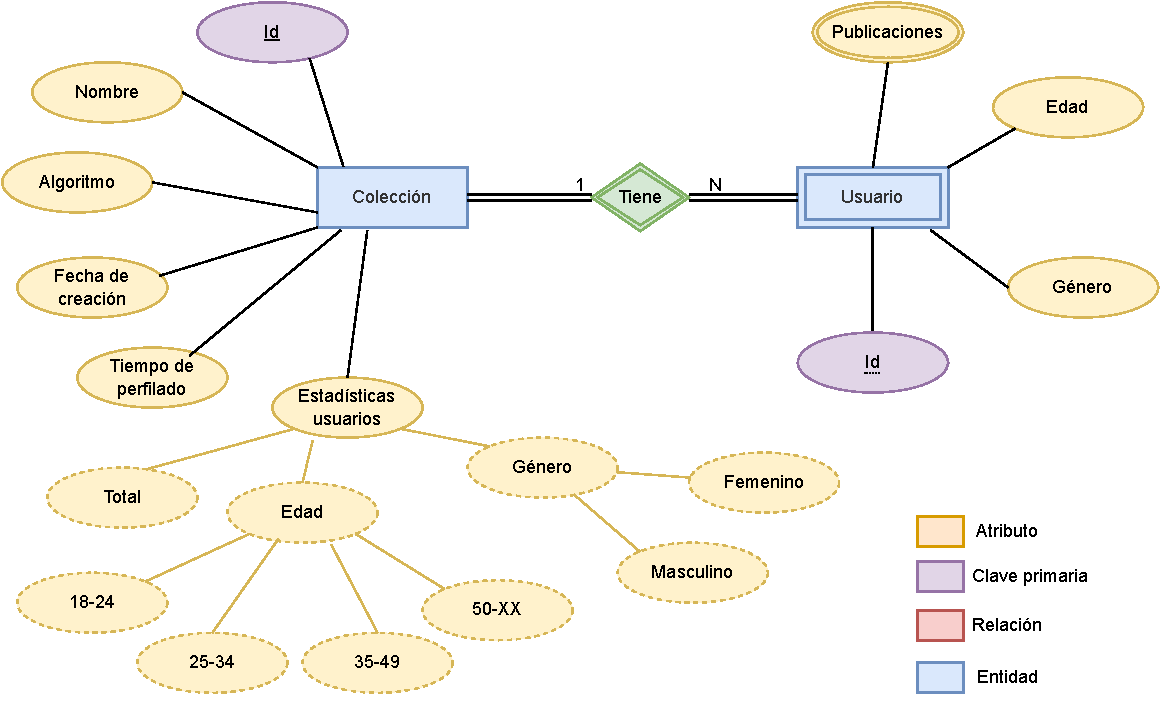
\includegraphics[width=\textwidth]{imaxes/diagramas/ER-diagram.pdf}
  \caption{Diagrama de entidad-relación del sistema.}
  \label{fig:diagrama/ER}
\end{figure}

Como se puede observar se tienen únicamente dos entidades fundamentales relacionadas entre sí: \textit{Colección} y \textit{Usuario}. 
% \begin{itemize}
%     \item \textbf{\textit{Colección}}: esta entidad representa una colección de usuarios ya perfilada
% \end{itemize}